\documentclass[11pt]{article}
\usepackage{amsmath}
\usepackage{amssymb}
\usepackage{graphicx}
\usepackage{natbib}
\usepackage{lineno}
\usepackage{color} 
\usepackage{setspace} 
\topmargin 0.0cm
\oddsidemargin 0.5cm
\evensidemargin 0.5cm
\textwidth 16cm 
\textheight 21cm
\usepackage[labelfont=bf,labelsep=period,justification=raggedright]{caption}
\makeatletter
\renewcommand{\@biblabel}[1]{\quad#1.}
\makeatother
\date{}
\pagestyle{myheadings}
\newcommand{\ie}{{\em i.e.}, }
\newcommand{\eg}{{\em e.g.}, }
\newcommand{\CiteP}[1]{(\citeauthor{#1}, \citeyear{#1})}
\newcommand{\CiteT}[1]{\citeauthor{#1} (\citeyear{#1})}
\newcommand{\Cite}[1]{\citeauthor{#1}, \citeyear{#1}}


\begin{document}

\thispagestyle{empty}
{\Large
\centerline{\textbf{After the games are over: }}
\centerline{\textbf{decay of the Olympic Village effect following invasion}}
\centerline{\textbf{implies a trade-off between dispersal and fitness}}
\vspace{17 pt}

\large
\centerline{T. Alex Perkins$^{1}$, Carl Boettiger$^{2}$, Benjamin L. Phillips$^{3}$}}
\vspace{9 pt}

\begin{flushleft}
$^1$ Department of Biological Sciences and Eck Institute for Global Health, University of Notre Dame, Notre Dame, IN, USA, taperkins@nd.edu
$^2$ Center for Stock Assessment Research, University of California, Santa Cruz, CA, USA, cboettig@gmail.com
$^3$ Department of Zoology, University of Melbourne, Melbourne, VIC, Australia, phillipsb@unimelb.edu.au \\

\vspace{10 pt}
Keywords: competition; dispersal syndromes; evolution; fitness; invasion; life-history syndromes; range expansion; spatial spread; trade-off; traveling wave
\end{flushleft}


\subsection*{ABSTRACT}

Dispersal is apt to evolve upwards on invasion fronts due to assortative mating by dispersal, a phenomenon known as the ``Olympic Village effect'' or spatial sorting. But what happens after the invasion front has passed? Empirical and theoretical studies have suggested a decline in dispersal following invasion, but hypotheses about what drives this decline have not been clearly articulated or tested. Here we use a simple model of the spatiotemporal dynamics of two dispersal phenotypes to propose a general explanation. Following invasion, spatial sorting drives dispersal of its inhabitants downwards. This shift is fleeting, however, as a mixture of fast and slow phenotypes sets in as equilibrium densities are attained. Afterwards, dispersal only continues to evolve downwards if there is a trade-off between dispersal and fitness at high density. We conclude that empirical observations of declines in dispersal following invasion imply the existence of a trade-off between dispersal and fitness.


\subsection*{INTRODUCTION}

When a population spreads across space, several evolutionary forces come into play that should drive dispersal rates upwards on the invasion front (\Cite{Travis2002}; \Cite{Perkins2013}). First, under the Olympic Village effect \CiteP{Phillips2008a}, inhabitants at the farthest reaches of the invasion front tend to be limited to the most capable dispersers (\Cite{Shine2011a}; \Cite{Benichou2012}), leading to spatially assortative mating by dispersal capability and the perpetuation of this effect in subsequent generations \CiteP{Phillips2010}. More recently, this phenomenon has been referred to as ``spatial sorting,'' which we adopt henceforth. Second, in a density-regulated context, these highly dispersive phenotypes arriving on the invasion front benefit from a fitness advantage through lowered competition with conspecifics \CiteP{Phillips2008a}. Finally, this fitness advantage may increase over time, as reproduction also undergoes adaptive evolution in the vanguard population \CiteP{Perkins2013}.

Despite the fact that these evolutionary forces have only recently been elucidated, there is a rapidly growing body of empirical work showing that they often do result in increased dispersal on invasion fronts. Spreading populations ranging from trees to ants, crickets, beetles, and amphibians all show evidence of increased dispersal on the invasion front (\eg \Cite{Cwynar1987}; \Cite{Simmons2004c}; \Cite{Leotard2009}; \Cite{Alford2009}; \Cite{Lombaert2014}). These rapid increases in dispersal have broad implications for ecological management (\eg the management of invasive species, or native species shifting under climate change) and even medicine (\eg the growth of tumours, and the formation of biofilms) (\Cite{Orlando2013}; \Cite{VanDitmarsch2013}). While we are beginning to appreciate that dispersal evolves upwards on invasion fronts over time, we are much less clear about what happens to dispersal traits after the invasion front passes.

The evolutionary trajectory of dispersal after colonisation is important to understand for three reasons. First, it gives an indication of the long-term consequences of invasion on evolution. If the evolution of increased dispersal is a transient phenomenon and historical levels of dispersal quickly re-evolve following colonisation, then its long-term implications are modest. If, however, dispersal tends to be maintained at high levels following establishment, then a persistent cline in dispersal phenotypes will exist across the species' range, with implications for population dynamics and life-history evolution. In this case, invasion may also be a driver of diversification, with many instances of geographic variation being a product of past invasions \CiteP{Shine2011a} rather than local adaptation along an underlying environmental gradient \CiteP{Kirkpatrick1997}.

The second reason for understanding the post-colonisation trajectory of dispersal is that doing so potentially gives further insight into the processes occurring on the invasion front. Trade-offs between dispersal and fitness, for example, may alter the evolutionary and spread dynamics of the invasion front (\Cite{Burton2010}; \Cite{Orlando2013}). If such a trade-off exists, it may manifest as a rapid downward shift in dispersal behind the invasion front.  

Finally, and related to the first point, the reality is that the vast majority of well-documented examples of spread have more or less finished spreading (\Cite{Perkins2012}; Appendix F). Documenting the spread of an invasive species takes time -- time in which the population is filling its new range -- and so invasions are often only well-documented as they are reaching their conclusion. Because of this, our inference about evolutionary processes on invasion fronts will often be made by examining populations at numerous times post-colonisation; a kind of space for time substitution (\eg \Cite{Phillips2008a}). Do populations sampled $t$ years post-colonisation accurately represent phenotypes on the invasion front when it passed that location $t$ years ago, or do they represent phenotypes that have shifted substantially since then?

Here we attempt to provide clarity on the processes that govern the evolution of dispersal from the moment of colonisation onwards. It is clear from a handful of models and empirical studies that dispersal can evolve downward, from the elevated levels caused by invasion to lower levels following colonisation (\ie \Cite{Duckworth2007}; \Cite{Burton2010}; \Cite{Lindstrom2013}). Unfortunately, neither of these lines of evidence currently provides a clear indication as to why this happens, and therefore, how general that result is likely to be and what we can infer from it. Models that have investigated the evolutionary trajectory of dispersal post-colonisation tend to have been individual-based simulations in which mechanism can be difficult to pinpoint (\eg \Cite{Burton2010}; \Cite{Travis2010}). Any given empirical system will no doubt have its own peculiarities, too.

Discussion around these models and empirical examples suggest that there are, effectively, only two mechanisms that might cause dispersal to evolve downwards following colonisation: one spatial, the other temporal. The spatial mechanism is spatial sorting. Under this mechanism, dispersal phenotypes are sorted along the strong density cline on the invasion front (\Cite{Shine2011a}; \Cite{Benichou2012}). This moving density cline creates a situation in which the flow of dispersing individuals is asymmetric at any point along the cline; more individuals arrive from high-density areas than from low-density areas. This results in a positive net flow of less dispersive individuals into recently colonised areas and thus a downward shift in dispersal at a fixed location. The second mechanism influencing dispersal post-colonisation is the more familiar force of natural selection. If there is a trade-off between dispersal and fitness, then less dispersive individuals will tend to leave more offspring behind and so increase in frequency over time. 

Below, we develop a simple model and use it to determine the conditions under which these two mechanisms might operate following colonisation.  Developing the model at once clarifies the mechanisms, but also provides suggestions about the existence of trade-offs in spatially extended populations.


\subsection*{METHODS}

\subsubsection*{Model description}

We considered a species with two types: slow dispersers with density $N_s(t,x)$ at time $t$ and location $x$, and fast dispersers with density $N_f(t,x)$. For convenience, we dropped the notation indicating the specification of these variables over time and space. We assumed that each type disperses according to a diffusion process with mean squared displacement per time $D_s$ and $D_f$, respectively. At any particular location $x$ in the absence of immigration and emigration, we assumed that the population's density grows over time according to a logistic function, with growth rates $r_s$ and $r_f$ at low density and a shared carrying capacity $K$. Specifying population dynamics in this way resulted in the sum $N(t,x) = N_s(t,x) + N_f(t,x)$ at some $x$ obeying logistic growth.

Although the evolutionary dynamics of two such types could be modeled under a variety of genetic assumptions, we chose a simple formulation in which the fast and slow types have a one-to-one correspondence to two respective genotypes of a haploid organism. In most instances, we therefore assumed that offspring inherit their progenitor's genotype. In some instances, however, we allowed for either mutation, horizontal gene transfer, or recombination to effect a switch to the complementary genotype in the offspring. We allowed this switching to occur with probability $\mu$. The resulting dynamics are therefore similar to more complicated genetic models -- \eg a single-locus diploid model -- in that they allow for parents to produce offspring of both genotypes. A key distinction is that in alternative models, $\mu$ would depend on the relative frequencies of the genotypes, whereas in our model it does not.

The extent of interference competition within local populations was determined by coefficients $a_{fs}$ and $a_{sf}$, which dictated the impact of the density of each type on itself and on that of the other. Altogether, these assumptions resulted in the following equations,

\vspace*{-22pt}
\begin{subequations}
\begin{align}
\frac{\partial N_s}{\partial t} &= D_s \frac{\partial ^ 2 N_s}{\partial x ^ 2} + \mu r_f N_f + r_s N_s \left(1 - \mu - N_s / K - a_{fs} N_f / K \right) \label{dNsdt} \\
\frac{\partial N_f}{\partial t} &= D_f \frac{\partial ^ 2 N_f}{\partial x ^ 2} + \mu r_s N_s + r_f N_f \left(1 - \mu - N_f / K - a_{sf} N_s / K \right) \label{dNfdt},
\end{align}
\end{subequations}

\noindent which governed the dynamics of these types in time and space. The model was essentially a modified Lotka-Volterra model with a shared carrying capacity, potential for exchange between types through births, and spatial diffusion. We interpreted the logistic process as density-independent births minus density dependent deaths. This interpretation naturally leads $\mu$ to only be associated with the density-independent parts of the functions.

\subsubsection*{Nondimensionalization}

To reduce the number of parameters governing the dynamics of these types and to clarify the scales of interest for each variable, we nondimensionalized the model in eqq.~\eqref{dNsdt} and \eqref{dNfdt}. More background about the utility of this technique in ecology can be found in \CiteT{Petersen2001}. To apply this technique here, we first separated the dimensional and nondimensional components of each variable: $N_s = n_s N_s ^ *$, $N_f = n_f N_f ^ *$, $t = \tau t ^ *$, and $x = \chi x ^ *$. Substituting these separate components of each variable into eqq.~\eqref{dNsdt} and \eqref{dNfdt}, we obtained

\vspace*{-22pt}
\begin{subequations}
\begin{align}
\frac{\partial n_s}{\partial \tau} \frac{N_s^*}{t^*} &= D_s \frac{\partial ^ 2 n_s}{\partial \chi ^ 2} \frac{N_s^*}{{x^*}^2} + \mu r_f n_f N_f^* + r_s n_s N_s^* \left(1 - \mu - n_s N_s^* / K - a_{fs} n_f N_f^* / K \right) \label{dnNsdt} \\
\frac{\partial n_f}{\partial \tau} \frac{N_f^*}{t^*} &= D_f \frac{\partial ^ 2 n_f}{\partial \chi ^ 2} \frac{N_f^*}{{x^*}^2} + \mu r_s n_s N_s^* + r_f n_f N_f^* \left(1 - \mu - n_f N_f^* / K - a_{sf} n_s N_s^* / K \right) \label{dnNfdt}.
\end{align}
\end{subequations}

\noindent We then defined the dimensional components of the variables as $N_s^* = K$, $N_f^* = K$, $t^* = r_s ^ {-1}$, and $x^* = \sqrt{D_s/r_s}$, to obtain

\vspace*{-22pt}
\begin{subequations}
\begin{align}
\frac{\partial n_s}{\partial \tau} &= \frac{\partial ^ 2 n_s}{\partial \chi ^ 2} + \mu r n_f + n_s \left(1 - \mu - n_s - a_{fs} n_f \right) \label{dnsdt} \\
\frac{\partial n_f}{\partial \tau} &= D \frac{\partial ^ 2 n_f}{\partial \chi ^ 2} + \mu n_s + r n_f \left(1 - \mu - n_f - a_{sf} n_s \right) \label{dnfdt},
\end{align}
\end{subequations}

\noindent where $D = D_f / D_s$ and $r = r_f / r_s$.

\subsubsection*{Model analysis}

Our primary interest was understanding patterns of the relative frequencies of the fast and slow types across space following initial colonisation. Achieving this understanding required first determining the range of patterns that are possible and then how and why different ecological scenarios affect those patterns.

Because our interests were general and not in reference to any particular system, we limited our analyses to the nondimensionalized model in eqq. (3a) and (3b), which emphasizes relative differences between the two types. We analyzed this model primarily by solving it numerically under strategically chosen sets of parameter values. The initial conditions for the model were always $n_s=n_f=0.1$ at $\chi=0$ and $n_s=n_f=0$ elsewhere, and we solved the model on the domain $[0,35]_\chi\times[0,50]_\tau$. Additional parameter values used in obtaining specific results are noted in the figure captions.

All numerical analyses were performed in the R language \citep{R} and made use of the deSolve package \citep{deSolve}. In the interest of reproducibility and to facilitate exploration of model behavior under alternative parameter sets, the code for reproducing our results is available online at https://www.github.com/TAlexPerkins/dispersal\_tradeoffs. In addition to the numerical analyses, we performed some limited mathematical analyses of stability properties of equilibria of the model of local dynamics, which are documented in the Appendix.


\subsection*{RESULTS}

We first examined a model in which natural selection is absent and the only force operating on dispersal post-colonisation is spatial sorting.  Under this model -- in which population growth of each type was density-independent (\ie eqq. (3a) and (3b) without the quadratic terms), there is no trade-off, and no mutation -- dispersal evolved downwards after colonisation, approaching an even distribution of the two types (Fig. \ref{fcline_r}, top left panel, blue line). When we then introduced natural selection (\ie allowing $r<1$), the slow type approached displacement of the fast type (Fig. \ref{fcline_r}, top left panel, red line). The presence of mutation (\ie $\mu>0$) created an additional force pushing dispersal towards an even mixture of the types. Relative to alternative genetic models, this effect is somewhat exaggerated in our model because the mutation rate is density-independent, meaning that the more common type will produce more offspring of the less common type than it would otherwise. The net effect of higher mutation then is to hasten the downward shift of dispersal, but also to dampen the effect of the trade-off (Figs \ref{fcline_r}, \ref{ftime_r}, left).

Next, we examined a situation in which spatial sorting operates transiently.  Under this model -- in which population growth of each type displays negative density dependence, there is no trade-off, and no mutation -- dispersal evolved downwards until the population reached equilibrium density, at which point the mixture of fast and slow types stabilised (Figs \ref{fcline_r} \& \ref{ftime_r}, top right panel, blue line). When we introduced a trade-off in low-density population growth ($r<1$, Figs \ref{fcline_r} \& \ref{ftime_r}, top right panel, red line), dispersal evolved downwards very rapidly as a consequence of both spatial sorting and natural selection.  Interestingly, however, dispersal values once again appeared to stabilise at equilibrium density, despite the trade-off (Fig. \ref{ftime_r}).  This outcome is driven by the fact that, at equilibrium density, the population stops growing, and so a trade-off on $r$ makes no difference to the growth rate of either type.  As with the density-independent case, mutation acts as a force pushing the population towards an even mixture of the two types (Figs \ref{fcline_r}, \ref{ftime_r}, right).

Following these results, we then investigated the effect of a trade-off that limits the impact of interference by the fast type on the slow type.  Unlike the previous case (a trade-off on $r$), this trade-off becomes stronger as density increases. We first investigated the situation in which fast types exert weakened competitive interference on slow types ($a_{fs}=0.9$, Figs \ref{fcline_afs} \& \ref{ftime_afs}). In this situation, we again saw dispersal evolving downwards following colonisation (spatial sorting + trade-off), but then stabilising unless there is a trade-off (natural selection only, Figs \ref{fcline_afs} \& \ref{ftime_afs}, top row).  Because this trade-off operates even at equilibrium density, we saw dispersal evolving downward even after equilibrium density is attained, doing so more rapidly with a stronger trade-off (Figs \ref{fcline_afs} \& \ref{ftime_afs}, top row).  Once again, mutation had the effect of forcing trajectories towards an even mixture of the two types (Figs \ref{fcline_afs} \& \ref{ftime_afs}, rows 2-4). 

Finally, we investigated the situation in which slow types exert heightened competitive interference on fast types ($a_{sf}=1.1$).  This scenario had similar outcomes to the previous one, provided that the fast type did not also have a heightened ability to interfere with the slow type (Figs \ref{fcline_asf} \& \ref{ftime_asf}, right). In that case, the downward shift in dispersal stalled and a stable cline formed at an intermediate point beyond the invasion origin (Fig. \ref{fcline_asf}, top right). This situation is unique relative to the others that we evaluated because the local population dynamics under these parameter values are the only ones (in the absence of mutation or spatial effects) that are expected to converge on a stable equilibrium of coexistence between the two types (Appendix). As before, all of these effects eroded with increasing mutation (Fig. \ref{ftime_asf}, rows 2-4).


\subsection*{DISCUSSION}

When populations spread into new areas, dispersal will often evolve upwards on the invasion front as it moves forward (\Cite{Travis2002}; \Cite{Phillips2010}). But what happens to dispersal traits post-colonisation; \ie after the front has passed? If dispersal attenuates back to pre-invasion levels, why does this happen? Our model captures the two possible drivers of dispersal evolution in this scenario -- spatial sorting and natural selection -- and clarifies when and how they operate. A lack of clarity about this to date has impeded the interpretation of empirical results, which have typically assumed one mechanism over the other without fully considering both. A pattern of declining dispersal post-colonisation in bluebirds, for example, was attributed entirely to natural selection \CiteP{Duckworth2007}, whereas a similar pattern in cane toads was attributed to spatial sorting \CiteP{Lindstrom2013}. Rather than leave this determination to the proclivities of a study's authors, our goal is to establish a general understanding of how the processes of spatial sorting and natural selection give rise to these patterns in different contexts.

Both hypotheses about the drivers of declining dispersal behind invasion fronts appear to be partially true. Spatial sorting operates when there is a persistent density gradient on the invasion front. When we maintained this gradient in the model by allowing the population to grow in a density-independent manner, dispersal evolved downwards after colonisation, even in the absence of natural selection (\ie no trade-off between dispersal and fitness; Fig. \ref{ftime_r}, left). Thus, in the early stages of colonisation when population growth is exponential, spatial sorting is an important mechanism driving dispersal to lower levels. When we introduced density dependence into the model, but maintained a situation with no trade-off between dispersal and fitness, the mixture of fast and slow types ceased to change once an equilibrium density was attained (Fig. \ref{ftime_r}, right). In this equilibrium situation, dispersal effectively became a neutral trait. Thus, when a population attains an equilibrium density, spatial sorting ceases to operate and dispersal should remain frozen in time thereafter. When we introduced a trade-off between dispersal and fitness into the model with density dependence, dispersal evolved downwards again. Together, these scenarios suggest that the observation of declining dispersal after colonisation implies the existence of a trade-off between dispersal and fitness.

The role of any given trade-off in attenuating dispersal post-colonisation depends very much on whether it operates in a low- or high-density context. Trade-offs between dispersal and population growth at low density had no impact on the post-colonisation trajectory of dispersal in our model, although they would be expected to have substantial effects on spread dynamics \CiteP{Burton2010}. At high density, a trade-off between dispersal and interference competitive ability was the single most important determinant of the evolutionary fate of dispersal at a fixed location. Once a population reaches its carrying capacity locally, one phenotype must have some advantage over the other if a further shift in dispersal is to be effected. In reality, any trade-off between dispersal and a trait that confers a competitive advantage at high density (\eg exploitative competitive ability, longevity) could effect such a change. In applications spanning climate change to cancer, there is a large variety of particular trade-offs and ways in which these will interact (\Cite{Duputie2012}; \Cite{Aktipis2012}; \Cite{Orlando2013}). Nonetheless, in all these contexts, competition is likely an important force and so optimal strategies will vary between the invasion front and the core of the population. It has been hypothesised that one way for organisms to free up energy for increased dispersal and reproduction on an invasion front is to reduce investment in competition (\Cite{Burton2010}; \Cite{Phillips2010}); being a good competitor is less relevant in the low density conditions of the invasion front. Here, we see that such an evolutionary strategy ensures that dispersal will evolve to lower values after the invasion front passes. Thus, insofar as trading off competition for dispersal and reproduction is a general evolutionary outcome of invasion, evolution of lowered dispersal behind the invasion front will be a general outcome.

Our analysis also tempts the suggestion that by observing the trajectory of dispersal evolution over time at a recently colonised location, we might be able to infer things of interest such as a) the time to reach carrying capacity, b) the strength of spatial sorting, and c) the strength of natural selection.  Such an effort would have to be undertaken very cautiously, however. Before our approach could be reasonably used to make such nuanced inferences, the robustness of our results to a number of model assumptions would need to be evaluated more fully. For example, there are different potential models under which natural selection could enter the system (including kin selection; \Cite{Kubisch2013}), and genetic variation will also not be constant over time \CiteP{Polechova2009}. It would be valuable to know how these and other assumptions might alter our qualitative conclusions or, more likely, how they might yield different predictions about the shape and steepness of evolutionary trajectories of dispersal in time and space. Despite these limitations, contemporary measurements of dispersal and other phenotypes across space represent one of very few windows into the past that have the potential to inform us about the dynamics of bygone invasions, and we must have some theoretical basis for interpreting them.

Perhaps the strongest inference that can be drawn from our analysis is that if dispersal values evolve downwards following the attainment of equilibrium densities, then we can be confident about the operation of some sort of trade-off between dispersal and fitness at high density. Such trade-offs are often posited in theoretical models \CiteP{Ronce2007}, but empirical evidence of their existence is scarce (primarily coming from flight-fecundity trade-offs in insects; \eg \Cite{Hughes2003b}). A primary reason for this paucity of examples is that it is logistically difficult to measure relevant variables (life-history and dispersal traits) and then to be sure that all relevant life-history traits have been taken into account (\Cite{Ronce2007}; \Cite{Phillips2010}). Negative relationships between fecundity and dispersal, for example, could be cancelled out by negative correlations between fecundity and age to maturity, which would go undetected unless all traits are measured.  Observation of post-colonisation declines in dispersal provide a new way of inferring the existence of such a trade-off, even if the proximate traits remain unidentified. By following the evolutionary trajectory of the dispersal trait after colonisation, we can gain clear insight into whether or not a trade-off is in operation.


\subsection*{CONCLUSION}

Our analysis suggests that dispersal typically only returns to equilibrium levels following colonisation when there is a trade-off between dispersal and fitness. If these trade-offs are prevalent in nature, then the long-term implications of dispersal evolution during invasion are likely modest. Gradients in dispersal across the invaded range will, in the absence of alternative fitness peaks, be transient phenomena, and diversification of life-histories driven by spread may be unusual. Additionally, where there are trade-offs, dispersal phenotypes at a location do not reflect the phenotypes that first colonised that location, but will be less dispersive phenotypes that have evolved following colonisation. Thus, the existence or otherwise of trade-offs is a critical thing to know about.  Although we don't really know how prevalent trade-offs between dispersal and fitness are in nature, we now have a new way of looking for them.


\subsection*{ACKNOWLEDGEMENTS}

We would like to thank Rick Shine, Greg Brown, and Vincent Calvez for useful discussion around these ideas.  TAP received support from the Research and Policy for Infectious Disease Dynamics (RAPIDD) program of the Science and Technology Directory, Department of Homeland Security, and Fogarty International Center, National Institutes of Health. CB was supported by NSF DBI-1306697, and BLP was supported by the Australian Research Council's Fellowships program (DP1094646).


\bibliographystyle{bibstyle}
\bibliography{references}


\subsection*{APPENDIX}

\subsubsection*{Equilibria for local population dynamics}

First, we limited this analysis of equilibria to the case where $\mu=0$. Then, after removing the diffusion terms and examining the dynamics of an isolated population with the local population dynamics defined in eqq.~\eqref{dnsdt} and \eqref{dnfdt}, we found four equilibria. The first was the trivial equilibrium wherein neither type is present: \ie $\overline{n}_s = 0$ and $\overline{n}_f = 0$. The second and third were $(\overline{n}_f, \overline{n}_s)=(0,1)$ and $(1,0)$, respectively. The fourth was a coexistence equilibrium found by solving the system of equations

\vspace*{-22pt}
\begin{subequations}
\begin{align}
n_s + a_{fs} n_f & = 1 \\
n_f + a_{sf} n_s & = 1,
\end{align}
\end{subequations}

\noindent which yielded

\vspace*{-22pt}
\begin{subequations}\label{equilib}
\begin{align}
\overline{n}_s & = \frac{a_{fs} - 1}{a_{fs} a_{sf} - 1} \\
\overline{n}_f & = \frac{a_{sf} - 1}{a_{fs} a_{sf} - 1} .
\end{align}
\end{subequations}

\noindent It should be noted that one important set of parameter values for which the equlibrium in eq.~\eqref{equilib} is undefined is when $a_{fs} = a_{sf} = 1$. In this case, any combination of values of $n_s$ and $n_f$ such that $n_s + n_f = 1$ is an equilibrium.

\subsubsection*{Local asymptotic stability of the equilibria}

For a given equilibrium $(\overline{n}_s,\overline{n}_f)$, we can determine local asymptotic stability (LAS) about that equilibrium by determining whether the Jacobian matrix

\begin{equation}
J = \left( \begin{array}{cc}
	1-2\,\overline{n}_s-a_{fs}\overline{n}_f & -a_{fs}\overline{n}_s \\
	-ra_{sf}\overline{n}_f & r(1-2\,\overline{n}_f-a_{sf}\overline{n}_s) \\
	\end{array} \right)
\end{equation}

\noindent evaluated at $(\overline{n}_s,\overline{n}_f)$ has two eigenvalues with negative real parts. A sufficient and necessary condition for LAS is that the determinant of $J$ is positive and that its trace is negative.

\noindent \textit{Case 1}: $\overline{n}_s=0,\overline{n}_f=0$

In this case, $\textrm{det}(J)=r$ and $\textrm{tr}(J)=1+r$. Therefore, the equilibrium is not LAS because satisfying both criteria involves a contradiction.

\noindent \textit{Case 2}: $\overline{n}_s=0,\overline{n}_f=1$

In this case, $\textrm{det}(J)=r(a_{fs}-1)$ and $\textrm{tr}(J)=1-a_{fs}-r$. Therefore, the equilibrium is LAS if $a_{fs}>1$.

\noindent \textit{Case 3}: $\overline{n}_s=1,\overline{n}_f=0$

In this case, $\textrm{det}(J)=r(a_{sf}-1)$ and $\textrm{tr}(J)=-1-r(a_{sf}-1)$. Therefore, the equilibrium is LAS if $a_{sf}>1$.

\noindent \textit{Case 4}: $\overline{n}_s=(a_{fs} - 1)/(a_{fs} a_{sf} - 1),\overline{n}_f=(a_{sf} - 1)/(a_{fs} a_{sf} - 1)$

In this case, 

\vspace*{-22pt}
\begin{subequations}
\begin{align}
\textrm{det}(J) &= \frac{r(a_{fs}-1)(a_{sf}-1)}{a_{fs}a_{sf}-1} \\
\textrm{tr}(J) &= -1-r(a_{sf}-1) .
\end{align}
\end{subequations}

\noindent If $0 < a_{fs} < 1$ and $0 < a_{sf} < 1$, then the equilibrium is LAS if $r > a_{fs} + a_{sf} - 1$. If $0 < a_{sf} < 1$ and $a_{fs}>1$, then the equilibrium is LAS if $a_{fs}a_{sf} > 1$ and $a_{fs} > r - a_{sf} + 1$. If $0 < a_{fs} < 1$ and $a_{sf}>1$, then the equilibrium is LAS if $a_{fs}a_{sf} > 1$. Finally, if $a_{fs} > 1$ and $a_{sf} > 1$, then the equilibrium is LAS.


\newpage
\subsection*{FIGURES}

\begin{figure}[!ht]
\begin{center}
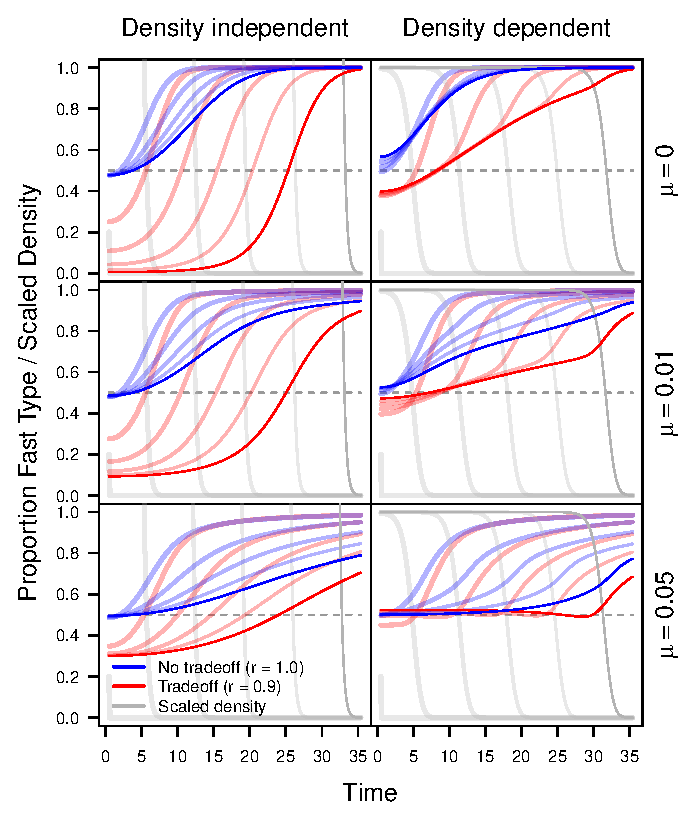
\includegraphics[width=4.68in]{../output/clines_r.pdf}
\end{center}
\caption{
Effects of density dependence (columns) and relative growth rate at low density ($r$) on the proportion of fast types across space at multiple time points. Values of the mutation rate ($\mu$) vary across rows. Lines of the same color represent spatial patterns sampled in successive increments of $10$ time units from left to right. Blue is the situation of no trade-off, whereas red denotes a trade-off on $r$. Population density (scaled to a maximum of one) is shown in gray. Initial frequencies of each type were even, and relative dispersal ability $D=1.2$. An even frequency is shown by the dashed line.
}
\label{fcline_r}
\end{figure}

\begin{figure}[!ht]
\begin{center}
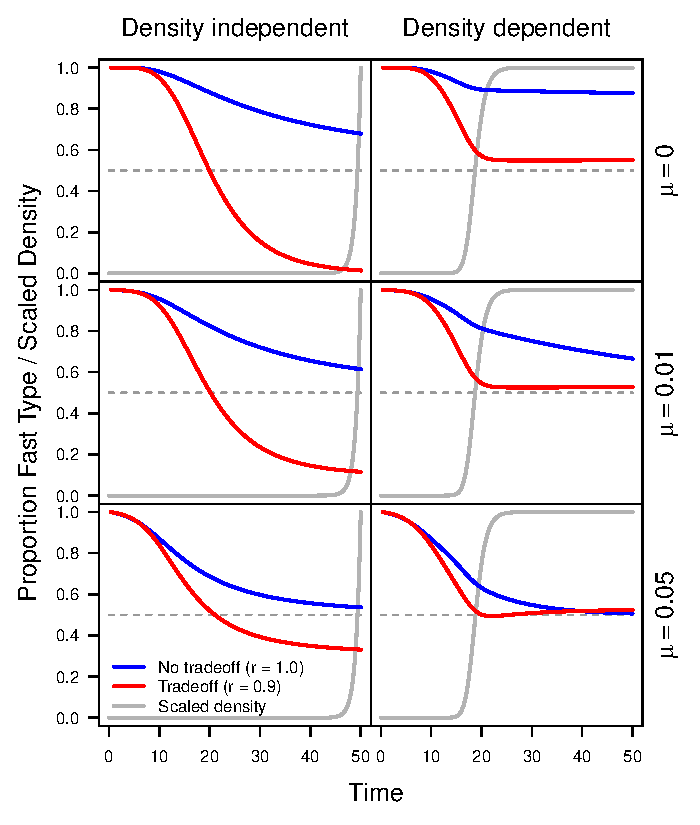
\includegraphics[width=4.68in]{../output/time_r.pdf}
\end{center}
\caption{
The evolutionary trajectory of dispersal after colonisation is affected by density dependence (columns) and a trade-off on relative growth rate at low density ($r$, colored lines). The vertical axis shows the proportion of fast phenotypes at $x=10$ over time. Values of the mutation rate ($\mu$) vary across rows. Relative dispersal ability $D=1.2$, and initial frequencies of the types were even at introduction. Population density over time (scaled to a maximum of one) is shown in the solid grey line of the background. 
}
\label{ftime_r}
\end{figure}

\begin{figure}[!ht]
\begin{center}
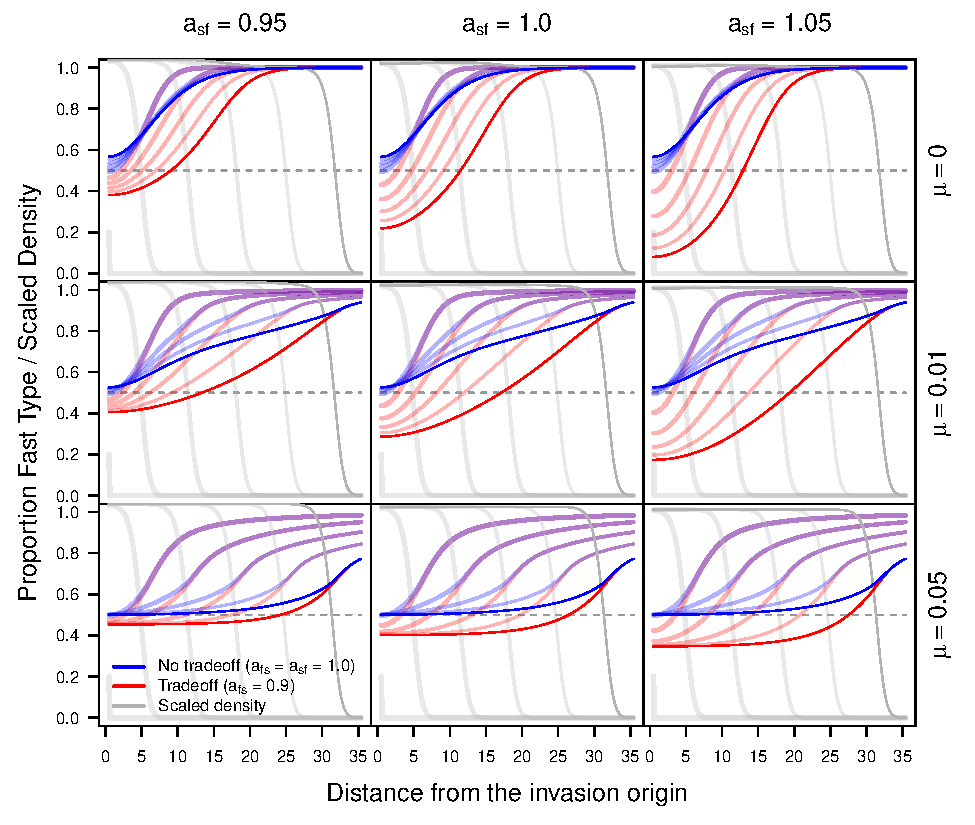
\includegraphics[width=4.68in]{../output/clines_afs.pdf}
\end{center}
\caption{
Effects of interference competition by the slow type on the fast type ($a_{sf}$, columns) and vice versa ($a_{fs}$, colored lines) on the proportion of fast types across space at multiple time points. Values of the mutation rate ($\mu$) vary across rows. Lines of the same color represent spatial patterns sampled in successive increments of $10$ time units from left to right. Blue is the situation of no trade-off, whereas red denotes a trade-off on $a_{fs}$. Population density (scaled to a maximum of one) is shown in gray. Initial frequencies of each type were even, and relative dispersal ability $D=1.2$. An even frequency is shown by the dashed line.
}
\label{fcline_afs}
\end{figure}

\newpage
\begin{figure}[!ht]
\begin{center}
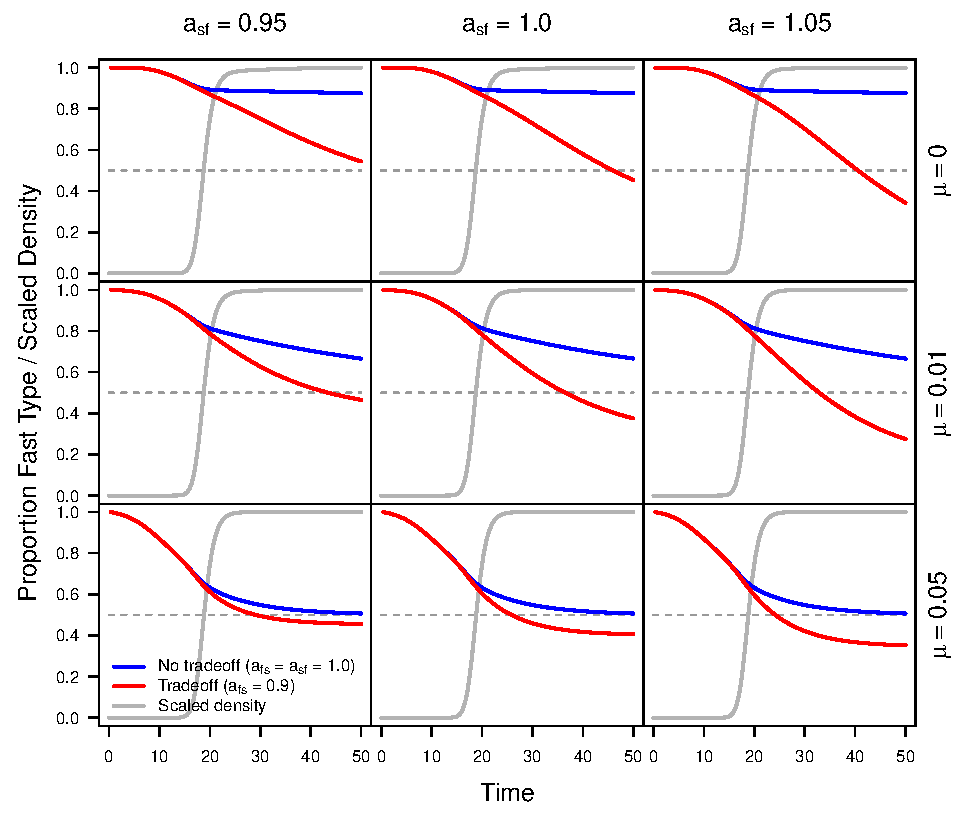
\includegraphics[width=6.5in]{../output/time_afs.pdf}
\end{center}
\caption{
The evolutionary trajectory of dispersal after colonisation is affected by interference competition by the slow type on the fast type ($a_{sf}$, columns) and vice versa ($a_{fs}$, colored lines). The vertical axis shows the proportion of fast phenotypes at $x=10$ over time. Values of the mutation rate ($\mu$) vary across rows. Relative dispersal ability $D=1.2$, and initial frequencies of the types were even at introduction. Population density over time (scaled to a maximum of one) is shown in the solid grey line of the background. 
}
\label{ftime_afs}
\end{figure}

\begin{figure}[!ht]
\begin{center}
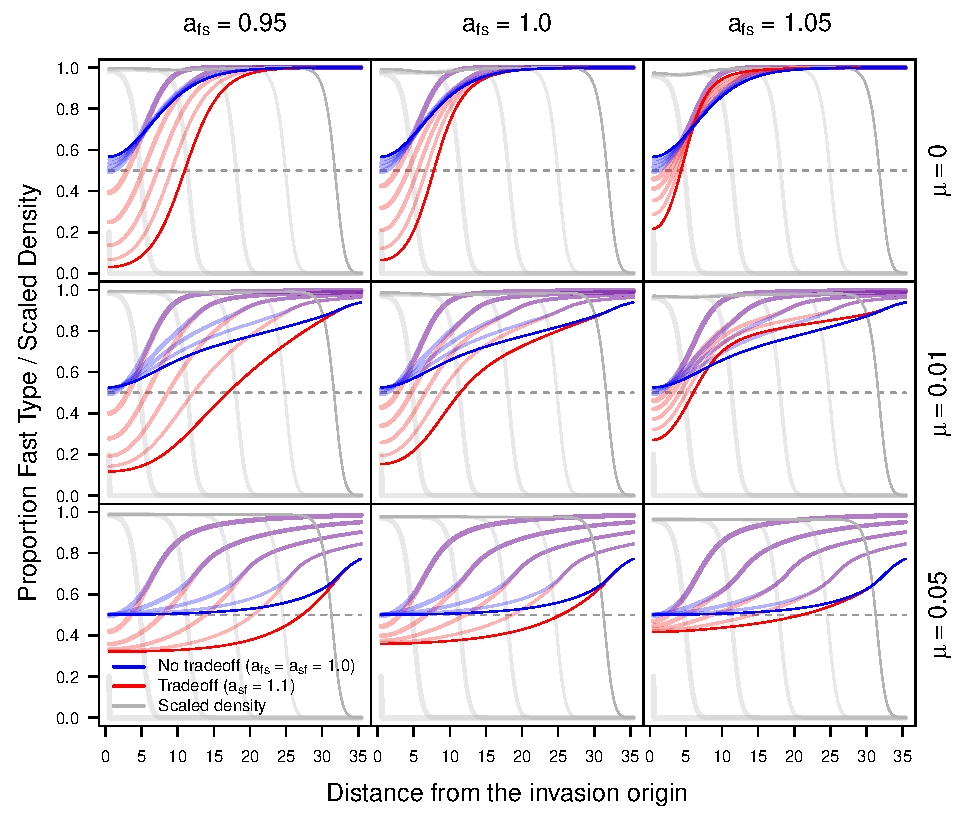
\includegraphics[width=4.68in]{../output/clines_asf.pdf}
\end{center}
\caption{
Effects of interference competition by the fast type on the slow type ($a_{fs}$, columns) and vice versa ($a_{sf}$, colored lines) on the proportion of fast types across space at multiple time points. Values of the mutation rate ($\mu$) vary across rows. Lines of the same color represent spatial patterns sampled in successive increments of $10$ time units from left to right. Blue is the situation of no trade-off, whereas red denotes a trade-off on $a_{sf}$. Population density (scaled to a maximum of one) is shown in gray. Initial frequencies of each type were even, and relative dispersal ability $D=1.2$. An even frequency is shown by the dashed line.
}
\label{fcline_asf}
\end{figure}

\newpage
\begin{figure}[!ht]
\begin{center}
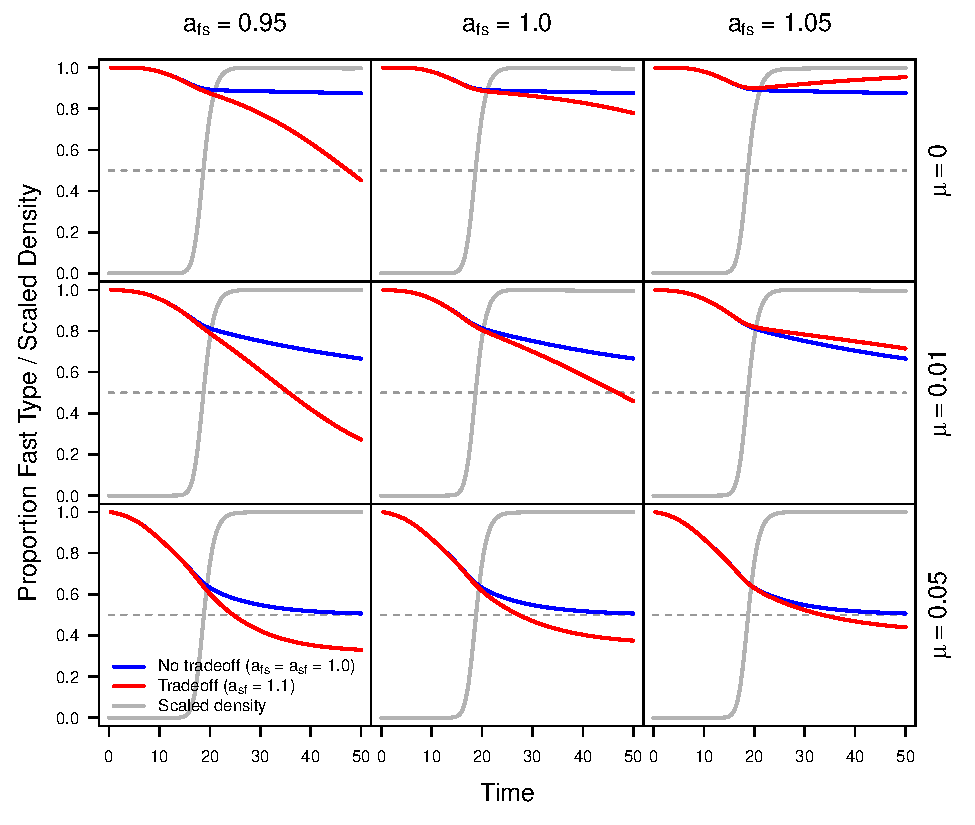
\includegraphics[width=6.5in]{../output/time_asf.pdf}
\end{center}
\caption{
The evolutionary trajectory of dispersal after colonisation is affected by interference competition by the fast type on the slow type ($a_{fs}$, columns) and vice versa ($a_{sf}$, colored lines). The vertical axis shows the proportion of fast phenotypes at $x=10$ over time. Values of the mutation rate ($\mu$) vary across rows. Relative dispersal ability $D=1.2$, and initial frequencies of the types were even at introduction. Population density over time (scaled to a maximum of one) is shown in the solid grey line of the background. 
}
\label{ftime_asf}
\end{figure}


\end{document}
